

\part*{Lezione (27/11/2025)}

\section{Confronto Ordinamenti}
\subsection*{Riepilogo Complessità}

\begin{center}
    \textbf{Ordine di grandezza del:}

    \vspace{0.2cm}
    $\swarrow \quad \searrow$
    \vspace{0.2cm}

    \begin{tabular}{|l|c|c|c|c|l|}
        \hline
        \multirow{3}{*}{\textbf{Algoritmo}} & \multicolumn{3}{c|}{\textbf{COSTO IN TEMPO}} & \multirow{2}{*}{\textbf{COSTO}} & \multirow{3}{*}{\textbf{Commenti}} \\
        & \multicolumn{3}{c|}{} & \multirow{2}{*}{\textbf{IN SPAZIO}} & \\ \cline{2-4}
        & \shortstack{CASO \\ OTTIMO} & \shortstack{CASO \\ MEDIO} & \shortstack{CASO \\ PESSIMO} & & \\
        \hline
        Insertion Sort & $n$ & $n^2$ & $n^2$ & in loco & \\
        \hline
        Selection Sort & $n^2$ & $n^2$ & $n^2$ & in loco & \\
        \hline
        Merge Sort & $n \log n$ & $n \log n$ & $n \log n$ & $n$ & OTTIMO in tempo \\
        \hline
        Quick Sort & $n \log n$ & $n \log n$ & $n^2$ & \shortstack{in loco \\ + gestione \\ RICORSIONE} & \shortstack{OTTIMO in tempo \\ al caso medio} \\
        \hline
        \textbf{Heapsort} & $n \log n$ & $n \log n$ & $n \log n$ & in loco & \shortstack{OTTIMO in tempo \\ e spazio} \\
        \hline
    \end{tabular}
\end{center}

\vspace{0.3cm}
\noindent
$\llcorner \!\! \rightarrow$ \textbf{Heapsort} utilizza una struttura dati specifica: lo \textbf{HEAP}.

\hrulefill

\section{Struttura Dati: HEAP (di Massimo)}

\subsection{Definizione}
L'Heap rappresenta un \textbf{albero binario quasi completo}.
\begin{itemize}
    \item \textbf{Quasi completo} significa che l'albero è riempito completamente in tutti i livelli, tranne eventualmente l'ultimo.
    \item Sull'ultimo livello, i nodi sono tutti \textbf{accumulati a sinistra}.
\end{itemize}

\subsection{Rappresentazione in Array}
Anche se concettualmente è un albero, l'Heap viene solitamente rappresentato utilizzando un \textbf{array}.
\begin{itemize}
    \item Non serve memorizzare puntatori espliciti a padre e figli.
    \item La mappatura dall'albero all'array avviene tramite una \textbf{visita per livelli} (breadth-first).
    \item La radice si trova in $A[0]$.
    \item Gli elementi successivi seguono l'ordine della visita.
\end{itemize}

\noindent
Sia $A.heap\_size$ il numero di elementi dell'heap memorizzati in $A$. Gli elementi validi dell'heap si trovano negli indici da $0$ a $A.heap\_size - 1$.

\subsection{Regole di Posizionamento (Indici)}
Dato un nodo $x$ che corrisponde all'elemento di indice $i$ nell'array $A$:

\begin{center}
    \begin{tikzpicture}[
        node distance=1cm,
        level distance=1.2cm,
        sibling distance=2cm,
        every node/.style={circle, draw, minimum size=0.6cm, inner sep=0pt},
        arr_cell/.style={rectangle, draw, minimum width=1cm, minimum height=0.6cm, inner sep=0pt}
        ]

        % Disegno Albero
        \node[dashed] (t) {$t$}
        child {
        node (x) {$x$} edge from parent[dashed]
        child { node (y) {$y$} edge from parent[solid]}
        child { node (z) {$z$} edge from parent[solid]}
        };

        % Etichetta nodo x
        \node[draw=none, right=0.1cm of x] {\footnotesize \textit{indice $i$}};

        % Disegno Array sotto
        \node[arr_cell, below=2cm of t, xshift=-2cm] (arr_t) {$t$};
        \node[arr_cell, right=0cm of arr_t] (arr_x) {$x$};
        \node[arr_cell, right=0cm of arr_x, minimum width=1.5cm] (dots) {$\dots$};
        \node[arr_cell, right=0cm of dots] (arr_y) {$y$};
        \node[arr_cell, right=0cm of arr_y] (arr_z) {$z$};
        \node[arr_cell, right=0cm of arr_z, minimum width=1cm] (end) {};

        % Etichette indici array
        \node[below=0.1cm of arr_t, draw=none] {\footnotesize $\lfloor \frac{i-1}{2} \rfloor$};
        \node[below=0.1cm of arr_x, draw=none] {\footnotesize $i$};
        \node[below=0.1cm of arr_y, draw=none] {\footnotesize $2i+1$};
        \node[below=0.1cm of arr_z, draw=none] {\footnotesize $2i+2$};

        % Frecce o linee di collegamento logico (opzionale)
        \draw[->, gray, dotted] (x) -- (arr_x);
    \end{tikzpicture}
\end{center}

\vspace{0.5cm}

\noindent
Le formule per navigare l'albero muovendosi tra gli indici dell'array sono:

\begin{align*}
    \textbf{Parent}(i) & \quad \longrightarrow \quad \text{return } \left\lfloor \frac{i-1}{2} \right\rfloor \\
    \textbf{Left}(i)   & \quad \longrightarrow \quad \text{return } 2i + 1 \\
    \textbf{Right}(i)  & \quad \longrightarrow \quad \text{return } 2i + 2
\end{align*}

\section{Proprietà degli Heap: Verifica ed Efficienza}

\subsection{Correttezza delle Regole di Posizionamento}
Possiamo verificare che le formule per navigare l'array siano coerenti. In particolare, applicando la funzione \texttt{Parent} al risultato di \texttt{Left} o \texttt{Right}, dobbiamo tornare al nodo di partenza $i$.

\begin{proof}[Verifica]
    Ricordiamo che $\text{Parent}(k) = \lfloor \frac{k-1}{2} \rfloor$.
    \begin{itemize}
        \item \textbf{Figlio Sinistro:} $k = 2i + 1$.
        \[ \text{Parent}(\text{Left}(i)) = \left\lfloor \frac{(2i + 1) - 1}{2} \right\rfloor = \left\lfloor \frac{2i}{2} \right\rfloor = i \]
        \item \textbf{Figlio Destro:} $k = 2i + 2$.
        \[ \text{Parent}(\text{Right}(i)) = \left\lfloor \frac{(2i + 2) - 1}{2} \right\rfloor = \left\lfloor \frac{2i + 1}{2} \right\rfloor = \left\lfloor i + 0.5 \right\rfloor = i \]
    \end{itemize}
    Le regole sono corrette: si "risale" esattamente al genitore.
\end{proof}

\subsection{Efficienza in Memoria (Spazio)}
Memorizzare l'heap in un vettore di dimensione $n$ è molto più efficiente rispetto a una rappresentazione esplicita con nodi e puntatori.
\begin{itemize}
    \item \textbf{Rappresentazione Array:} Richiede spazio $n$ (solo i dati).
    \item \textbf{Rappresentazione a Puntatori:} Richiederebbe spazio $3n$ (per ogni nodo: il dato + puntatore left + puntatore right + eventuale puntatore parent).
\end{itemize}

\section{Proprietà fondamentali}

\subsection{Proprietà di Max-Heap}
Un \textbf{Max-Heap} è un albero binario quasi completo che soddisfa la seguente invariante:

\begin{definition}[Max-Heap Property]
    Per ogni nodo $i$ diverso dalla radice ($i > 0$):
    \[ A[\text{Parent}(i)] \ge A[i] \]
    Ovvero: il valore di un nodo è sempre minore o uguale al valore del padre.
\end{definition}

\begin{observation}
    Da questa proprietà deriva che:
    \begin{enumerate}
        \item L'elemento massimo dell'intero heap si trova sempre nella radice ($A[0]$).
        \item In ogni sotto-albero, la radice del sotto-albero contiene il valore massimo tra tutti i nodi di quel sotto-albero.
    \end{enumerate}
\end{observation}

\subsection{Altezza e Profondità}
È fondamentale distinguere tra altezza e profondità dei nodi:
\begin{itemize}
    \item \textbf{Profondità (Depth) di un nodo:} La lunghezza del cammino (numero di archi) dalla radice al nodo. (La radice ha profondità 0).
    \item \textbf{Altezza (Height) di un nodo:} La lunghezza del cammino più lungo dal nodo a una foglia. (Le foglie hanno altezza 0).
    \item \textbf{Altezza dell'Heap ($h$):} Corrisponde all'altezza della radice, ovvero la massima distanza dalla radice a una foglia.
\end{itemize}

\part*{Proprietà Matematiche degli Heap}

Analizziamo le tre proprietà fondamentali che legano la dimensione dell'input $n$ alla struttura dell'albero.

\section*{1. Altezza dell'Heap}

\begin{property}
    Un heap di $n$ elementi ha altezza $h = \lfloor \log_2 n \rfloor$.
    In notazione asintotica:
    \[ h = O(\log n) \]
\end{property}

\begin{proof}[Dimostrazione]
    Consideriamo i limiti sul numero di nodi $n$ per un albero binario di altezza $h$:
    \begin{itemize}
        \item \textbf{Caso minimo:} L'albero è completo fino al livello $h-1$ e ha una sola foglia al livello $h$.
        \[ n \ge 2^h \]
        \item \textbf{Caso massimo:} L'albero è pieno (tutti i livelli completi fino ad $h$).
        \[ n \le 2^{h+1} - 1 < 2^{h+1} \]
    \end{itemize}
    Combinando le disuguaglianze otteniamo:
    \[ 2^h \le n < 2^{h+1} \]
    Applicando il logaritmo in base 2:
    \[ h \le \log_2 n < h+1 \]
    Poiché $h$ deve essere un intero, l'unica soluzione è:
    \[ h = \lfloor \log_2 n \rfloor \]
\end{proof}

\section*{2. Numero di Foglie}

\begin{property}
    Un heap di $n$ nodi contiene esattamente $\lceil n/2 \rceil$ foglie.
\end{property}

\begin{proof}[Dimostrazione]
    Possiamo derivare il numero di foglie sottraendo il numero di \textbf{nodi interni} dal totale $n$.
    Un nodo $i$ è un nodo interno se ha almeno un figlio (il sinistro). La condizione di esistenza del figlio sinistro è:
    \[ \text{Left}(i) < n \implies 2i + 1 \le n - 1 \]
    Risolvendo per $i$:
    \[ 2i \le n - 2 \implies i \le \frac{n}{2} - 1 \]
    Essendo $i$ un intero:
    \[ i \le \left\lfloor \frac{n}{2} \right\rfloor - 1 \]
    I nodi interni sono quindi quelli con indice da $0$ a $\lfloor n/2 \rfloor - 1$. Il loro numero è $\lfloor n/2 \rfloor$.
    Il numero di foglie è:
    \[ \#\text{foglie} = n - \#\text{interni} = n - \left\lfloor \frac{n}{2} \right\rfloor = \left\lceil \frac{n}{2} \right\rceil \]
\end{proof}

\section*{3. Nodi di Altezza $h$}

\begin{property}
    In un heap di $n$ nodi, ci sono al più:
    \[ \left\lceil \frac{n}{2^{h+1}} \right\rceil \]
    nodi di altezza $h$.
\end{property}

\begin{intuition}[Caso dell'Albero Pieno - ABCB]
    Consideriamo un \textbf{ABCB} (Albero Binario Completamente Bilanciato), ovvero un heap "pieno" su tutti i livelli.
    Sia $H$ l'altezza totale dell'albero. Il numero totale di nodi è:
    \[ n = 2^{H+1} - 1 \]
    Analizziamo il numero di nodi per ogni altezza $h$:
    \begin{itemize}
        \item \textbf{Altezza $h=0$ (Foglie):} Circa metà dei nodi sono foglie ($n/2$).
        \item \textbf{Altezza $h=1$ (Padri delle foglie):} Sopra le foglie c'è un livello con la metà dei nodi rispetto al livello 0 ($n/4$).
        \item \textbf{Altezza generica $h$:} Generalizzando, il numero di nodi decresce esponenzialmente con l'altezza: $\approx n/2^{h+1}$.
    \end{itemize}
\end{intuition}

\part*{Manutenzione dell'Heap}

\section{Procedura MAX-Heapify}

\subsection{Definizione e Scopo}
\begin{definition}[MAX-Heapify]
    La procedura \texttt{MAX-Heapify} è un algoritmo fondamentale utilizzato per ripristinare la proprietà di Max-Heap in un nodo specifico che potrebbe violarla.
\end{definition}

\noindent
\textbf{Precondizioni (Ipotesi):}
Affinché la procedura funzioni correttamente, assumiamo che gli alberi binari radicati in $\text{Left}(i)$ e $\text{Right}(i)$ siano già dei \textbf{Max-Heap}, mentre $A[i]$ potrebbe essere minore dei suoi figli.

\subsection{Esempio Grafico}
L'indice $i=1$ (valore $4$) viola la proprietà perché è minore del figlio sinistro ($14$).

\vspace{0.5cm}

\begin{center}
    \begin{tikzpicture}[
        level distance=1.5cm,
        sibling distance=2cm,
        every node/.style={circle, draw, minimum size=0.8cm},
        highlight/.style={fill=red!20, draw=red, thick},
        arrow_line/.style={->, thick, red, bend right=45}
        ]
        % --- DISEGNO DELL'ALBERO ---
        \node (n0) {16}
        child { node[highlight] (n1) {4} % Nodo che viola
        child { node[highlight] (n3) {14} % Figlio maggiore
        child { node (n7) {2} }
        child { node (n8) {8} }
        }
        child { node (n4) {7}
        child { node (n9) {1} }
        child[missing]
        }
        }
        child { node (n2) {10}
        child { node (n5) {9} }
        child { node (n6) {3} }
        };
        % Frecce e label
        \node[draw=none, right=0.1cm of n1, red] {\footnotesize $i=1$};
        \node[draw=none, left=0.1cm of n3, red] {\footnotesize max};
        \draw[<->, dashed, thick, red] (n1) -- (n3) node[midway, right] {\footnotesize swap};

        % --- DISEGNO DELL'ARRAY ---
        \begin{scope}[yshift=-6cm, xshift=-4cm]
            \node[draw=none, rectangle] at (0, 0.8) {\textbf{Rappresentazione Array:}};
            \foreach \x/\val in {0/16, 1/4, 2/10, 3/14, 4/7, 5/9, 6/3, 7/2, 8/8, 9/1} {
            \node[draw, rectangle, minimum size=0.8cm] (arr\x) at (\x, 0) {\val};
            \node[draw=none, below=0.1cm of arr\x] {\footnotesize \x};
            }
            \node[draw=red, thick, rectangle, minimum size=0.8cm] at (1, 0) {4};
            \node[draw=red, thick, rectangle, minimum size=0.8cm] at (3, 0) {14};
            \draw[->, thick, red] (arr1.south) to[out=-45, in=-135] (arr3.south);
        \end{scope}
    \end{tikzpicture}
\end{center}

\subsection{Pseudocodice}

\begin{algorithm}
    \caption{MAX-Heapify(A, i)}
    \begin{algorithmic}[1]
        \State $l \gets \text{Left}(i)$
        \State $r \gets \text{Right}(i)$
        \State $max \gets i$
        \State \Comment{Controlla se il figlio sinistro esiste ed è maggiore del corrente massimo}
        \If{$l < A.heap\_size \textbf{ and } A[l] > A[max]$}
            \State $max \gets l$
        \EndIf
        \State \Comment{Controlla se il figlio destro esiste ed è maggiore del corrente massimo}
        \If{$r < A.heap\_size \textbf{ and } A[r] > A[max]$}
            \State $max \gets r$
        \EndIf
        \State \Comment{Se il massimo non è la radice $i$, scambia e ricorri}
        \If{$max \neq i$}
            \State \textbf{swap} $A[i] \leftrightarrow A[max]$
            \State \textsc{Max-Heapify}$(A, max)$
        \EndIf
    \end{algorithmic}
\end{algorithm}

\subsection{Analisi della Complessità}

\begin{analysis}[Costo Temporale]
    Il costo è proporzionale all'altezza del nodo $i$, poiché nel caso peggiore il valore scende fino alle foglie.
    \[ T(n) = O(h) = O(\log n) \]
\end{analysis}

\hrulefill

\section{Costruzione dell'Heap (Build-Max-Heap)}

\subsection{Strategia Bottom-Up}
La procedura trasforma un array disordinato in un Max-Heap chiamando \texttt{Max-Heapify} a ritroso, dai nodi interni fino alla radice.
Le foglie (da $\lfloor n/2 \rfloor$ a $n-1$) sono già heap validi.

\begin{center}
    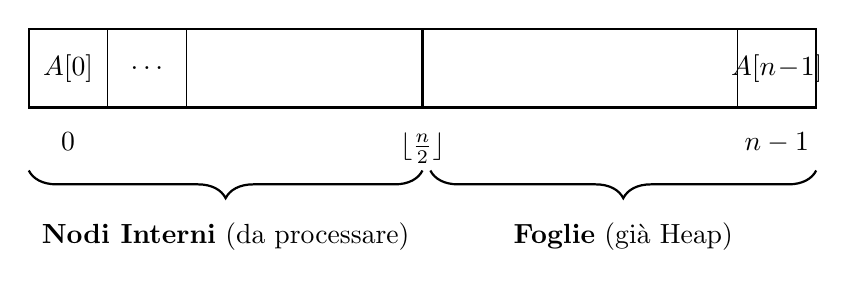
\begin{tikzpicture}[scale=1]
        \draw[thick] (0,0) rectangle (10, 1);
        \draw (1,0) -- (1,1); \node at (0.5, 0.5) {$A[0]$}; \node at (1.5, 0.5) {$\dots$}; \draw (2,0) -- (2,1);
        \draw[thick] (5,0) -- (5,1);
        \draw (9,0) -- (9,1); \node at (9.5, 0.5) {$A[n\!-\!1]$};
        \node[below=0.2cm] at (0.5,0) {$0$};
        \node[below=0.2cm] at (5,0) {$\lfloor \frac{n}{2} \rfloor$};
        \node[below=0.2cm] at (9.5,0) {$n-1$};
        \draw[decorate, decoration={brace, amplitude=10pt, mirror}, thick] (0,-0.8) -- (5,-0.8) node[midway, below=15pt] {\textbf{Nodi Interni} (da processare)};
        \draw[decorate, decoration={brace, amplitude=10pt, mirror}, thick] (5.1,-0.8) -- (10,-0.8) node[midway, below=15pt] {\textbf{Foglie} (già Heap)};
    \end{tikzpicture}
\end{center}

\subsection{Pseudocodice}

\begin{algorithm}
    \caption{Build-Max-Heap(A)}
    \begin{algorithmic}[1]
        \State $A.heap\_size \gets A.length$
        \For{$i \gets \lfloor \frac{A.length}{2} \rfloor - 1 \textbf{ downto } 0$}
            \State \textsc{Max-Heapify}$(A, i)$
        \EndFor
    \end{algorithmic}
\end{algorithm}

\section{Analisi della Complessità di Build-Max-Heap}

\subsection{Analisi Accurata}
Il costo totale non è $O(n \log n)$, ma \textbf{lineare} $O(n)$.
Il costo totale $T(n)$ è la somma dei costi per ogni nodo, che dipendono dall'altezza $h$.
\[ T(n) = \sum_{h=0}^{\lfloor \log n \rfloor} (\text{nodi di altezza } h) \times O(h) \]
Sostituendo il numero massimo di nodi $\lceil n/2^{h+1} \rceil$:
\[ T(n) \le \frac{c \cdot n}{2} \sum_{h=0}^{\lfloor \log n \rfloor} \frac{h}{2^h} \]
La serie $\sum \frac{h}{2^h}$ converge a 2. Pertanto:
\[ T(n) \le \frac{c \cdot n}{2} \cdot 2 = O(n) \]


\section*{Correttezza}

\subsection{Invariante di ciclo}

All'inizio dell'iterazione del ciclo for...

\section{Analisi del Costo in Tempo}

Limite superiore:
$n/2$ chiamate di \textsc{Max-Heapify}...

\newpage





















